\documentclass{standalone}
\usepackage{tikz}

\begin{document}

	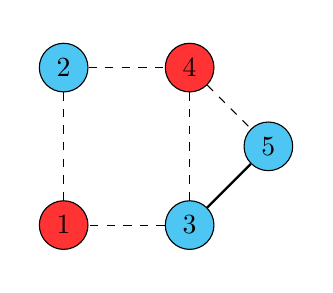
\begin{tikzpicture}[rotate=90]
		% Nodes
		\node[draw,circle,fill=red!80] (1) at (1,.8) {1};
		\node[draw,circle,fill=cyan!70] (2) at (3,.8) {2};
		\node[draw,circle,fill=cyan!70] (3) at (1,-.8) {3};
		\node[draw,circle,fill=red!80] (4) at (3,-.8) {4};
		\node[draw,circle,fill=cyan!70] (5) at (2,-1.8) {5};
		
		% Edges
		\draw[dashed] (1) -- (2)-- (4) -- (3) -- (1);
		\draw[dashed] (4) -- (5);
		\draw[thick] (3) -- (5);
		
		% Blanks
		\draw[<->, color=white] (.5,1.25) -- (.5,-2.25);
		\draw[<->, color=white] (3.5,0.35) -- (3.5,-0.35);
		
	\end{tikzpicture}

\end{document}